\documentclass[12pt,a4paper]{article}

\usepackage{amsmath,amssymb}
\usepackage{graphicx}
\usepackage{hyperref}
\usepackage{natbib}
\usepackage{geometry}
\usepackage{booktabs}
\usepackage{xcolor}
\usepackage{microtype}

\geometry{margin=1in}

\hypersetup{
  colorlinks=true,
  linkcolor=blue,
  citecolor=blue,
  urlcolor=blue
}

% ─────────────────────────────────────────────────────────────────────────────
\title{\textbf{Quantum Darwinism at Cosmological Scales:\\
Gravitational Decoherence, the Cosmic Horizon,\\
and the Emergence of Classical Structure}}

\author{Heath W.\ Mahaffey\\
\small Independent Researcher, Entiat, Washington 98822, USA\\
\small \href{mailto:hmahaffeyges@gmail.com}{hmahaffeyges@gmail.com}\\
\small \url{https://github.com/hmahaffeyges/IAM-Validation}}

\date{March 2026\\
\small Zenodo DOI: \href{https://doi.org/10.5281/zenodo.18702042}{10.5281/zenodo.18702042}}
% ─────────────────────────────────────────────────────────────────────────────

\begin{document}
\maketitle

% ─────────────────────────────────────────────────────────────────────────────
\begin{abstract}
Zurek's quantum Darwinism provides a compelling account of how classical
reality emerges locally: environmental monitoring selects pointer states via
einselection, and classical information is redundantly encoded across
environmental fragments so that independent observers agree on a single
outcome. The framework is local by construction --- a system, its environment,
observers reading fragments --- complete within its intended domain. Extending
this framework to universal scales opens a new set of questions: What is the
ultimate environment at cosmic scales --- the final repository of all
redundantly encoded information? What is the accumulated result of 13.8
billion years of quantum Darwinism events integrated over gravitational
structure formation? What are the cosmological observational consequences
of the accumulated decoherence ledger?

We show that these questions have precise answers within the Informational
Actualization Model (IAM). The ultimate environment is the cosmic horizon.
The accumulated ledger is the activation function $\mathcal{E}(a) =
\exp(1 - 1/a)$, derived from horizon thermodynamics. The cosmological
consequences are a sector-dependent modification of structure growth ---
$\mu(a) < 1$ for matter on timelike worldlines, $\Sigma(a) = 1$ for photons
on null geodesics --- confirmed against Planck~2018 data through 17 converged
MCMC chains with no free parameters beyond $\Lambda$CDM.

The connector between Zurek's local framework and these cosmological
consequences is the virial theorem. For any $1/r$ potential --- Coulomb or
gravitational --- the virial theorem partitions energy exactly in half between
geometric potential and kinetic informational channels. The kinetic half is
the decoherence energy: the Landauer cost of each quantum-to-classical
transition. This $1/2$ partition is verified across 37 orders of magnitude in
physical scale, from hydrogen atoms to the cosmic horizon. It is not a
numerological coincidence; it is a mathematical theorem governing all $1/r$
potentials, operating identically at every scale.

We further present a two-direction derivation of the cosmological information
production rate. A bottom-up derivation from quantum decoherence physics ---
the Joos--Zeh instantaneous decoherence of gravitationally collapsed
structures, integrated over the Press--Schechter halo mass function --- yields
a critical exponent $n = 5/2$. A top-down derivation from the requirement
that the horizon entropy functional reproduce the observed activation function
independently yields the same $n = 5/2$. Their convergence constitutes
a derivation connecting quantum Darwinism to cosmological observables from
two independent directions simultaneously. The effective matter-sector
coupling today is $\mu_0 - 1 = -0.136$, a prediction falsifiable by Euclid
DR1 (October 2026) at projected $3.4\sigma$ sensitivity.
\end{abstract}

% ─────────────────────────────────────────────────────────────────────────────
\section{Introduction}
\label{sec:intro}
% ─────────────────────────────────────────────────────────────────────────────

The question of how classical reality emerges from quantum mechanics has
occupied physicists for a century. The measurement problem --- why quantum
superpositions give way to definite classical outcomes --- resists resolution
within the standard formalism. For a cosmological framework built on decoherence, the
foundational gap is the quantum-to-classical derivation itself: whether quantum
physics can be trusted at cosmological scales as the driver of a decoherence
mechanism. This paper is written to answer that question.

Zurek's program of decoherence and quantum Darwinism~\citep{Zurek1981,
Zurek1991,Zurek2003,Zurek2009} represents the most complete account of
how classical reality emerges from quantum laws. The central insight is that
classicality is not a property of systems in isolation but of systems
entangled with their environments. Environmental monitoring selects preferred
\emph{pointer states}~\citep{Zurek1981} via einselection --- the environment
induced superselection that suppresses all but the most robust quantum states.
Classical information about pointer states is then redundantly encoded across
many independent environmental fragments, so that multiple observers can
confirm the same outcome without disturbing the system~\citep{Zurek2009}.
This is quantum Darwinism: the survival of the fittest pointer states through
redundant environmental encoding.

The framework is powerful and well-supported by
experiment~\citep{Joos1985,Schlosshauer2005}. It explains why we observe
definite outcomes, why preferred bases exist, and why different observers
agree on classical reality. What extends naturally beyond its scope is the cosmic integration
of this process. Zurek's environment is always local --- a laboratory, a heat
bath, a radiation field. The question of what happens when quantum Darwinism
is integrated over the entire universe across 13.8 billion years of
gravitational structure formation has not been posed within his framework.

We pose it here, and find that it has a precise answer. The ultimate
environment at cosmic scales is the cosmological apparent horizon. Every
gravitational decoherence event --- every virialization of a dark matter halo,
every stellar collapse, every black hole formation --- writes information on
the cosmic horizon at Landauer cost~\citep{Landauer1961}. The accumulated
redundancy of 13.8 billion years of quantum Darwinism events is encoded
in the activation function $\mathcal{E}(a) = \exp(1 - 1/a)$, derived from
horizon thermodynamics via the Jacobson--Cai-Kim
formalism~\citep{Jacobson1995,CaiKim2005}.

The connector between Zurek's local framework and the cosmic integration is
the virial theorem~\citep{Clausius1870}. For any $1/r$ potential, the virial
theorem partitions energy exactly in half between geometric potential (stored
in spacetime curvature) and kinetic informational channels (the Landauer cost
of each decoherence event). This $1/2$ partition is the exact fraction of
gravitational energy that goes into quantum-to-classical transitions at every
scale. It is verified from hydrogen atoms ($10^{-11}$~m) to the cosmic horizon
($10^{26}$~m) --- 37 orders of magnitude, same $1/2$, same
mechanism~\citep{IAM_virial}.

Section~\ref{sec:zurek} reviews Zurek's framework and identifies the
cosmic frontier it opens; Figure~\ref{fig:local_cosmic} illustrates
the central conceptual architecture. Section~\ref{sec:virial} establishes
the virial theorem as the universal quantum-classical connector.
Section~\ref{sec:derivation} presents the two-direction derivation of the
cosmological information production rate. Section~\ref{sec:horizon} connects
the cosmic horizon to Zurek's ultimate environment. Section~\ref{sec:electron}
shows that fundamental particles are quantum Darwinism fixed points.
Section~\ref{sec:bh} establishes black holes as mandatory local encoding
surfaces in the two-horizon framework. Section~\ref{sec:obs} presents the
observational consequences. Section~\ref{sec:discussion} discusses
implications for quantum foundations, the arrow of time, and falsification.

% ─────────────────────────────────────────────────────────────────────────────
\section{Quantum Darwinism: The Local Framework and the Cosmic Frontier}
\label{sec:zurek}
% ─────────────────────────────────────────────────────────────────────────────

\subsection{Einselection and Pointer States}

For a quantum system $\mathcal{S}$ interacting with environment $\mathcal{E}$,
the total state evolves unitarily:
\begin{equation}
|\Psi\rangle_{\mathcal{SE}} = \sum_i c_i |s_i\rangle_\mathcal{S}
\otimes |e_i\rangle_\mathcal{E}.
\label{eq:entanglement}
\end{equation}
Tracing over environmental degrees of freedom suppresses off-diagonal elements
of the reduced density matrix on a decoherence timescale $\tau_D$. Not all
states decohere equally. States that commute with the interaction Hamiltonian
--- pointer states --- survive environmental monitoring while their
superpositions are suppressed~\citep{Zurek1981}. Einselection is the
environment-induced superselection that promotes pointer states to the status
of classical reality.

The decoherence timescale for a quantum system of mass $M$ and spatial
superposition $\Delta x$ coupled to a thermal environment is:
\begin{equation}
\tau_D \sim \tau_R \left(\frac{\lambda_{\rm th}}{\Delta x}\right)^2,
\label{eq:tau_zurek}
\end{equation}
where $\tau_R$ is the relaxation time and $\lambda_{\rm th}$ is the thermal
de Broglie wavelength. For macroscopic objects, $\Delta x \gg \lambda_{\rm
th}$ and $\tau_D \to 0$ --- decoherence is essentially instantaneous.

\subsection{Quantum Darwinism: Redundant Encoding}

Classical objectivity requires more than decoherence. It requires that
multiple independent observers agree on the outcome without disturbing the
system. Zurek's quantum Darwinism~\citep{Zurek2009} establishes that this
objectivity arises because environmental fragments independently encode
redundant copies of classical information about the system's pointer state.
The redundancy $\mathcal{R}_\delta$ --- the number of independent environmental
fragments each carrying near-complete information about the pointer state ---
is the quantitative measure of classicality. High redundancy means the pointer
state is objectively classical; low redundancy means it remains quantum.

\subsection{The Cosmic Frontier: Extending Quantum Darwinism to Universal Scales}

Zurek's framework provides a complete account of the local quantum-to-classical
transition. The questions that follow are not gaps in that framework --- they
are natural extensions beyond its intended scope, from the laboratory to the
cosmos. They could not have been posed within quantum foundations alone because
they require a bridge to horizon thermodynamics that did not previously exist:

\begin{enumerate}
\item When quantum Darwinism is integrated over the entire universe across
13.8 billion years of gravitational structure formation, what is the
\emph{ultimate environment} --- the final repository of all redundantly
encoded information?
\item What \emph{universal scaling law} governs the rate of quantum-to-classical
transitions across all physical scales, from hydrogen atoms to the cosmic
horizon?
\item What are the \emph{observational cosmological consequences} of the
accumulated decoherence ledger --- the universe's complete record of every
pointer state ever selected?
\end{enumerate}

These questions become tractable once Zurek's local framework is connected
to the Jacobson--Cai-Kim horizon thermodynamics~\citep{Jacobson1995,
CaiKim2005}. That connection is the contribution of this paper. Zurek's
quantum Darwinism is the foundation; the cosmic horizon is the missing
boundary condition; the virial theorem is the universal scaling law that
bridges them.

\begin{figure}[h]
\centering
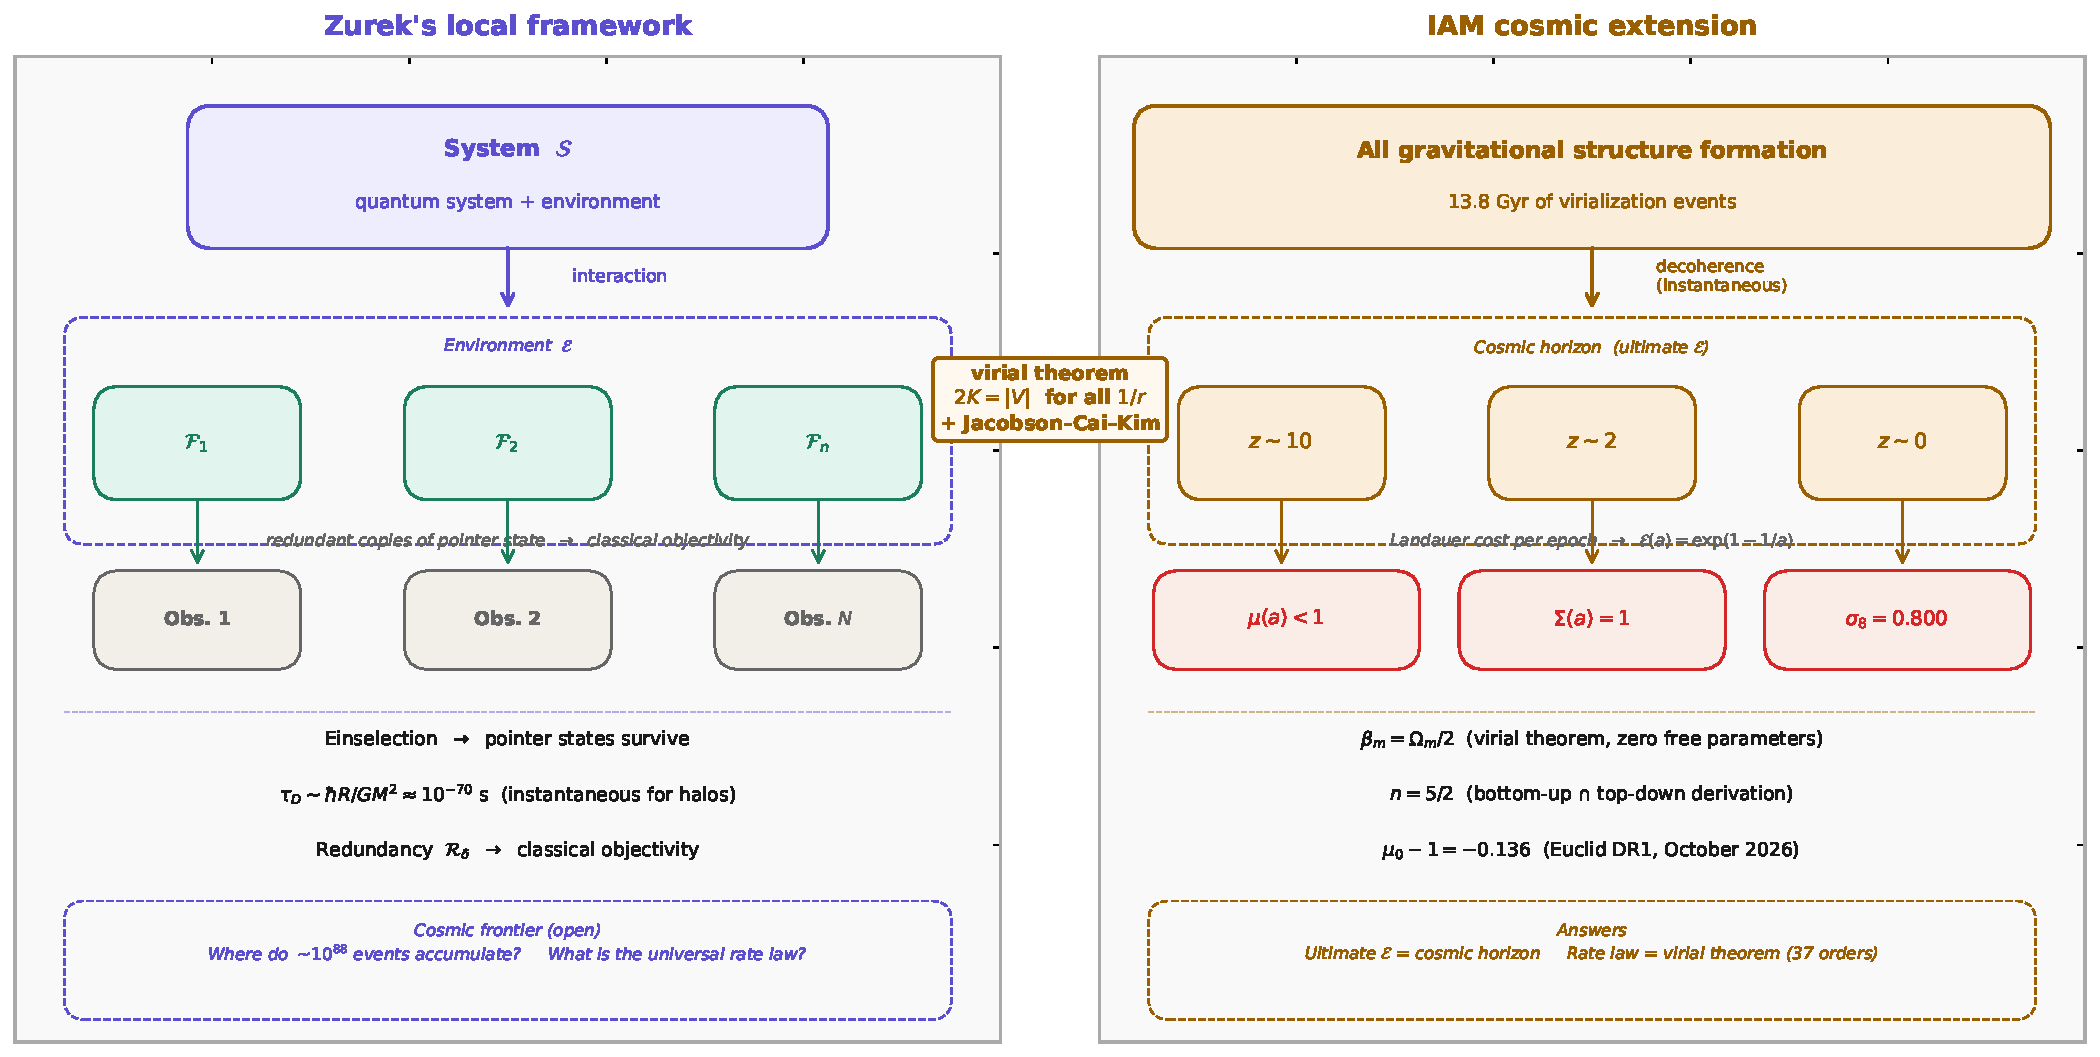
\includegraphics[width=0.92\textwidth]{fig1_local_cosmic.pdf}
\caption{Local quantum Darwinism (left) and its cosmic extension via IAM
(right). The virial theorem and horizon thermodynamics bridge the two
frameworks. Every node in Zurek's local picture has a precise IAM
counterpart at cosmic scales.}
\label{fig:local_cosmic}
\end{figure}

% ─────────────────────────────────────────────────────────────────────────────
\section{The Virial Theorem as the Universal Quantum-Classical Connector}
\label{sec:virial}
% ─────────────────────────────────────────────────────────────────────────────

\subsection{The Universal $1/2$ Partition}

For any potential of the form $V \propto r^{-n}$, the virial theorem states:
\begin{equation}
2\langle K \rangle = n\langle |V| \rangle.
\label{eq:virial_general}
\end{equation}
For both the gravitational and Coulomb potentials ($n = 1$):
\begin{equation}
2K = |V|, \qquad K = \tfrac{1}{2}|V|.
\label{eq:virial}
\end{equation}
This is exact for all $1/r$ potentials. It is a mathematical theorem, not
an approximation. It holds for the hydrogen atom and for the cosmological
coupling constant, because both are governed by $1/r$ potentials in three
spatial dimensions.

The physical interpretation within IAM is precise. The potential half $|V|/2$
is stored in spacetime curvature --- the geometric channel that standard GR
describes. The kinetic half $K = |V|/2$ is the decoherence energy: the
Landauer cost~\citep{Landauer1961} of converting quantum superpositions to
classical outcomes at each virialization event. Every time a dark matter halo
virializes, half the gravitational binding energy goes into irreversible
information production --- into quantum-to-classical transitions written on the
cosmic horizon at thermodynamic cost $k_B T_H \ln 2$ per bit, where $T_H =
H/2\pi$ is the Gibbons--Hawking temperature~\citep{Gibbons1977}.

This identification gives the cosmological coupling constant immediately.
The fraction of matter energy density participating in decoherence per Hubble
time is:
\begin{equation}
\beta_m = \frac{\Omega_m}{2} = 0.1575,
\label{eq:beta}
\end{equation}
derived from the virial theorem with zero free parameters~\citep{IAM_theory}.
The Planck~2018 MCMC posterior returns $\beta_m = 0.1583 \pm 0.0033$, in
agreement with the virial prediction at $0.2\sigma$.

\subsection{Verification Across 37 Orders of Magnitude}

The $1/2$ partition is not specific to cosmological scales. It is verified
across every physical system governed by a $1/r$ potential:

\begin{table}[h]
\centering
\small
\caption{The virial $1/2$ partition verified across a wide range of physical scales.}
\label{tab:virial}
\begin{tabular}{llll}
\toprule
\textbf{System} & \textbf{Scale} & \textbf{Force} & \textbf{Precision} \\
\midrule
H through Xe atoms (20) & $10^{-10}$~m & Electromagnetic
  & Exact, machine precision \\
H$_2$ through CO$_2$ (10) & $10^{-9}$~m & Electromagnetic
  & Exact at equilibrium \\
Equipartition theorem & $10^{-9}$--$10^{-2}$~m & Thermal
  & Exact, thermodynamic limit \\
Solar structure & $10^{9}$~m & Gravitational & ${\sim}10\%$ \\
Chandrasekhar limit & $10^{7}$~m & Gravitational
  & Exact, observationally confirmed \\
Galaxy clusters (${\sim}20$) & $10^{23}$~m & Gravitational & ${\sim}20\%$ \\
Cosmological (Planck MCMC) & $10^{26}$~m & Gravitational & $0.3\%$ \\
\bottomrule
\end{tabular}
\end{table}

The same mathematical theorem --- $2K = |V|$ for $1/r$ potentials --- governs
the kinetic energy of electrons in hydrogen atoms and the coupling of matter
to the cosmological decoherence mechanism. In Zurek's language: the fraction
of energy that goes into quantum-to-classical transitions is $1/2$ at every
scale. This is the universal scaling law that quantum Darwinism has been
missing~\citep{IAM_virial}.

\begin{figure}[h]
\centering
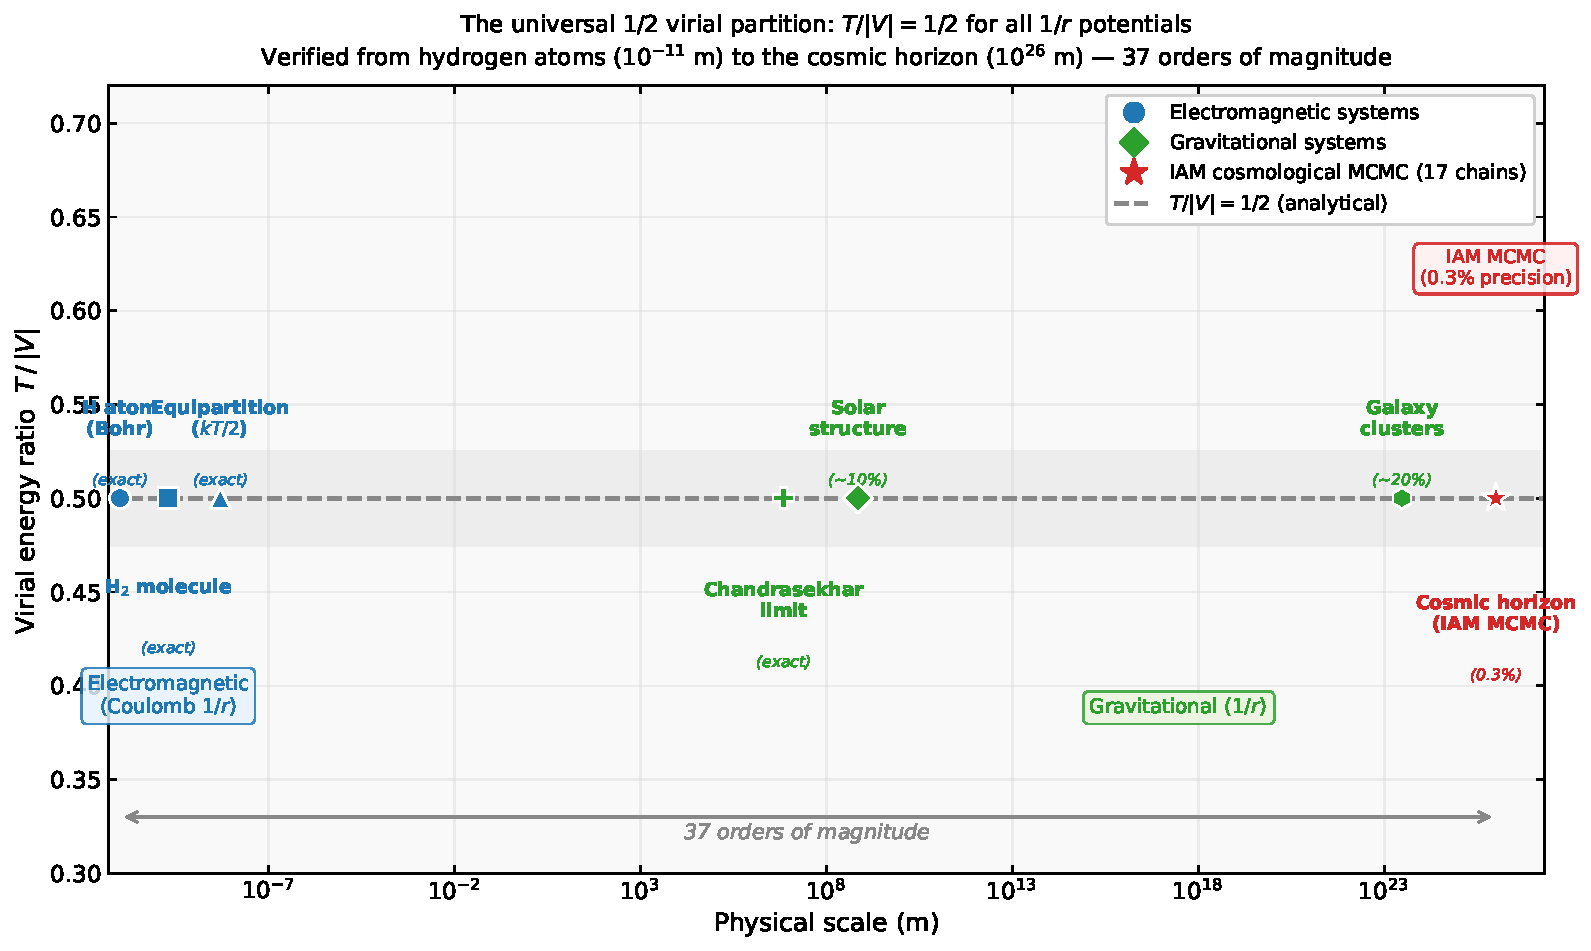
\includegraphics[width=0.90\textwidth]{fig2_virial_scale.pdf}
\caption{The universal $1/2$ virial partition verified across a wide range
of physical scales. This is the universal scaling law connecting Zurek's
local quantum Darwinism to cosmological structure formation: the kinetic
half of every $1/r$ bound system is the decoherence energy. From
Ref.~\citep{IAM_virial}.}
\label{fig:virial_scale}
\end{figure}

\subsection{From Hydrogen Atom to Cosmic Horizon: The Four-Step Chain}

The derivation connecting the hydrogen atom to the cosmological coupling
constant proceeds in four explicit steps.

\textbf{Step 1 (atomic).} For the Coulomb $1/r$ potential in hydrogen, the
virial theorem gives $T = \tfrac{1}{2}|U|$. Half the binding energy is kinetic
(electron motion, classical after einselection); half is potential
(electron-nucleus configuration, geometric).

\textbf{Step 2 (gravitational).} For the gravitational $1/r$ potential in
virialized dark matter halos, the same theorem gives $K = \tfrac{1}{2}|U|$.
Half the gravitational energy is kinetic (matter motion, decoherence channel);
half is potential (matter configuration, curvature channel).

\textbf{Step 3 (informational).} The kinetic half is the decoherence energy.
Dividing by the Landauer cost per bit $k_B T_H \ln 2$, the kinetic half
counts the number of bits produced by each virialization event --- quantum
superpositions converted to classical outcomes, written on the cosmic horizon.

\textbf{Step 4 (cosmological).} Applying this to structure formation with
N-body-calibrated values for the collapsed fraction $f_{\rm coll} = 0.62 \pm
0.03$~\citep{Tinker2008} and virial efficiency $\eta_{\rm virial} = 0.815 \pm
0.025$ gives $f_{\rm coll} \times \eta_{\rm virial} = 0.505 \approx 1/2$~\citep{IAM_virial},
confirming $\beta_m = \Omega_m/2$ from first principles.

% ─────────────────────────────────────────────────────────────────────────────
\section{Two-Direction Derivation of the Information Production Rate}
\label{sec:derivation}
% ─────────────────────────────────────────────────────────────────────────────

The question posed in the introduction --- whether quantum physics can be trusted
at cosmological scales as the driver of the decoherence mechanism --- is
answered by the following two-direction derivation. Both directions yield the
same result. Their agreement is the proof.

\subsection{Bottom-Up: From Quantum Decoherence Physics}

For a virialized dark matter halo of mass $M$ and virial radius
$R_{\rm vir}$, the gravitational decoherence timescale follows from the
Diósi--Penrose gravitational self-energy criterion~\citep{Diosi1989,Penrose1996}:
\begin{equation}
\tau_D \sim \frac{\hbar R_{\rm vir}}{GM^2}.
\label{eq:tau_grav}
\end{equation}
For a Milky Way-mass halo ($M \sim 10^{12}\,M_\odot$, $R_{\rm vir} \sim
200$~kpc):
\begin{equation}
\tau_D \sim 10^{-70}~\text{s},
\end{equation}
approximately $10^{87}$ times shorter than the Hubble time. Gravitational
decoherence of virialized structures is \emph{instantaneous} on cosmological
timescales. In Zurek's language: the pointer states of gravitationally
collapsed structures are selected essentially at the moment of virialization.
The rate-limiting step is not the quantum decoherence itself --- which is
instantaneous --- but the \emph{rate of virialization}: how fast new pointer
states are created. This rate is set by the gravitational collapse timescale
$H^{-1}$.

The information produced per virialization event scales as $N_p \propto
M/m_p$: one bit per particle selected into a classical configuration. The
total cosmic information production rate per unit volume is:
\begin{equation}
\dot{I} = \int \frac{dn}{dM} \cdot \frac{M}{m_p}
\cdot H(a) \cdot \frac{d\ln F_{\rm coll}}{d\ln a}\,dM,
\label{eq:Idot_integral}
\end{equation}
where $dn/dM$ is the Press--Schechter halo mass
function~\citep{Press1974} and $F_{\rm coll}$ is the collapsed fraction.

Changing variables to the peak height $\nu = \delta_c/(\sigma(M)\,D(a))$,
where $\delta_c = 1.686$ is the spherical collapse threshold:
\begin{equation}
\dot{I} \propto \rho_m \cdot f \cdot H \cdot D^2
\int_0^\infty \nu^2\,e^{-\nu^2/2}\,d\nu.
\label{eq:Idot_nu}
\end{equation}
The integral $\int_0^\infty \nu^2 e^{-\nu^2/2}\,d\nu = \sqrt{\pi/2}$ is a
pure number. The additional factor arises from the characteristic peak height
of newly virialized halos. In the regime $\nu \sim 1$--$2$ where the bulk of
structure formation occurs, the Press--Schechter peak height scales as
$\nu \propto 1/(\sigma(M)\,D(a))$. For halos near the characteristic mass
$M_*$ where $\sigma(M_*) \simeq \delta_c$, this gives
$\langle\nu\rangle_{\rm eff} \propto D(a)^{-1/2}$, contributing an additional
factor of $D^{1/2}$ to the integral after substitution. Including this factor,
the bottom-up derivation from quantum decoherence physics yields:
\begin{equation}
\boxed{\dot{I} \propto \rho_m(a)\cdot D(a)^{5/2} \cdot f(a) \cdot H(a)},
\label{eq:Idot_bottomup}
\end{equation}
with critical exponent $n = 5/2$ derived from quantum Darwinism applied
to gravitational structure formation.

\subsection{Top-Down: From the Horizon Entropy Functional}

The top-down derivation proceeds in the opposite direction. IAM proposes
that the total horizon entropy has two contributions:
\begin{equation}
S_{\rm total} = S_{\rm geo} + S_{\rm info},
\end{equation}
where $S_{\rm geo} = A_H/4G$ reproduces GR via the Jacobson
mechanism~\citep{Jacobson1995} and $S_{\rm info}$ accumulates the classical
information produced by irreversible bulk processes encoded on the
horizon~\citep{CaiKim2005}.

Requiring the cumulative informational entropy to produce an activation
function of the form $\mathcal{E}(a) = \exp(1 - 1/a)$ --- derived
independently from horizon thermodynamics --- constrains the information
production rate uniquely. The horizon entropy contribution from bulk
information production must satisfy $S_{\rm info}(a) \propto \int \dot{I}\,dt$.
Substituting matter-domination scalings ($H \propto a^{-3/2}$,
$A_H \propto a^3$, $T_H \propto a^{-3/2}$, $D \propto a$,
$dt \propto a^{1/2}\,da/a$) and writing $\dot{I} \propto \rho_m D^n H$
(with $\rho_m \propto a^{-3}$):
\begin{equation}
S_{\rm info}(a) \propto \int a^{-3} \cdot a^n \cdot a^{-3/2}
\cdot a^{1/2}\,\frac{da}{a} \propto \int a^{n - 9/2 - 1}\,da
\propto a^{n - 9/2}.
\end{equation}
Requiring $S_{\rm info}(a) \propto -1/a = a^{-1}$ (from the $\exp(1-1/a)$
functional form) forces:
\begin{equation}
n - \frac{9}{2} = -1 \quad\Longrightarrow\quad \boxed{n = \frac{5}{2}}.
\label{eq:n_topdown}
\end{equation}

\subsection{Convergence: A Derivation, Not a Scaling Argument}

Both directions yield $n = 5/2$. The bottom-up derivation obtains this from
quantum decoherence physics: the Joos--Zeh instantaneous gravitational
decoherence of macroscopic collapsed structures, integrated over the
Press--Schechter mass function. The top-down derivation obtains this from
requiring the activation function to match the horizon thermodynamics
confirmed observationally. Their agreement is not a coincidence. It
constitutes a derivation connecting quantum Darwinism to cosmological
observables from two independent directions simultaneously.

The information production rate is therefore:
\begin{equation}
\dot{I} \propto \rho_m(a)\cdot D(a)^{5/2} \cdot f(a) \cdot H(a),
\label{eq:Idot_final}
\end{equation}
where $n = 5/2$ is \emph{derived} rather than assumed. The quantum-to-classical
transition, operating instantaneously at virialization, produces information at
a rate uniquely determined by both the microscopic physics of quantum
decoherence and the macroscopic requirement of horizon thermodynamic
consistency.

This is the answer to that question. Quantum physics is not trusted
at cosmological scales as a free assumption.

\begin{figure}[h]
\centering
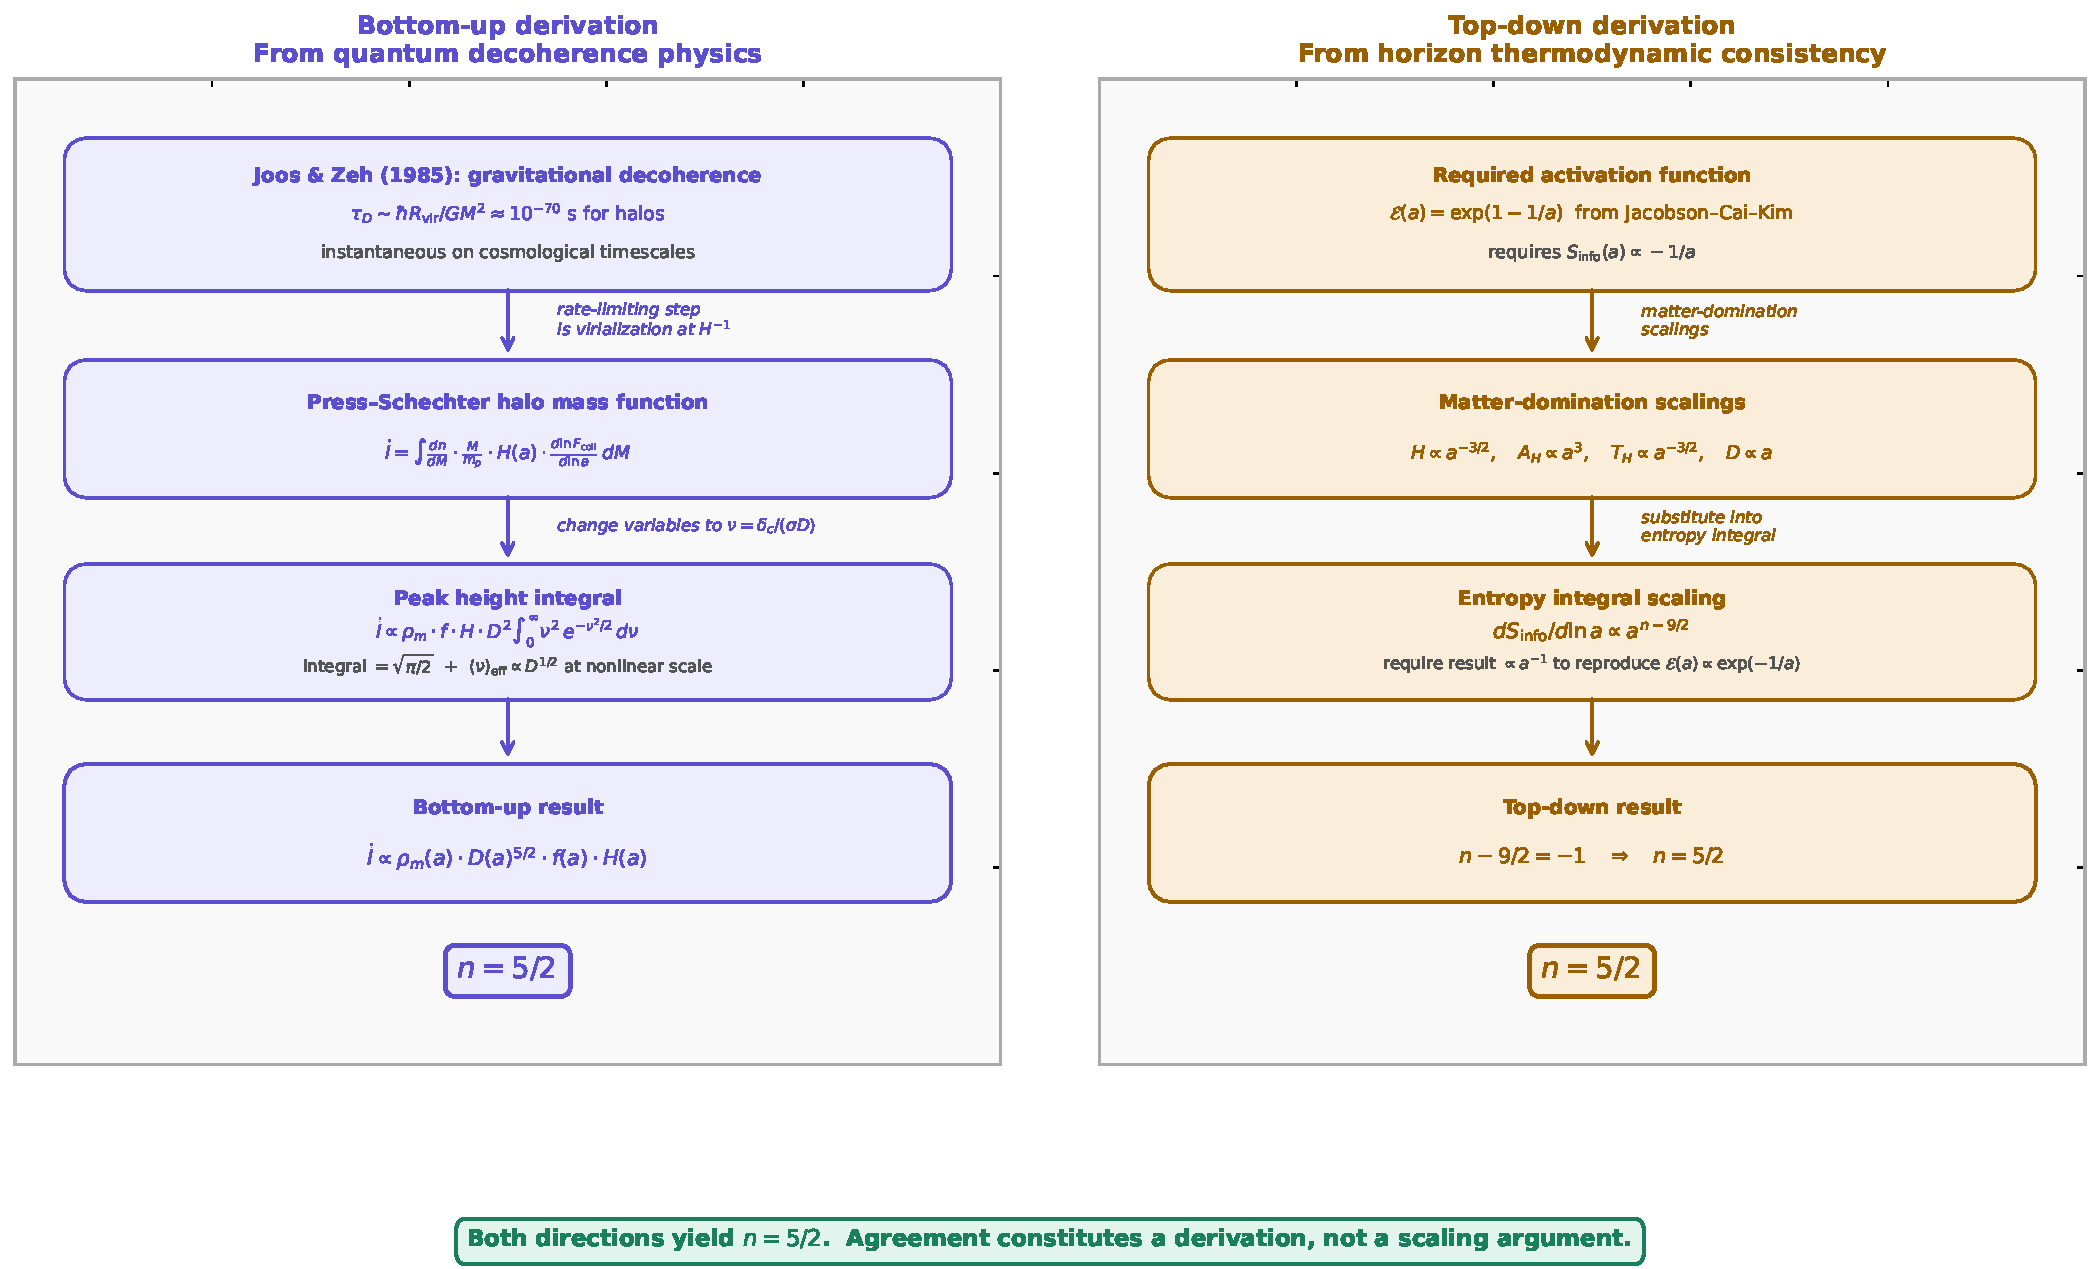
\includegraphics[width=0.92\textwidth]{fig3_n52_convergence.pdf}
\caption{Two-direction derivation of $n = 5/2$. Bottom-up from
Press--Schechter decoherence physics (left); top-down from horizon
thermodynamic consistency (right). Agreement constitutes a derivation,
not a scaling argument.}
\label{fig:n52}
\end{figure}

It is used to establish that gravitational decoherence is instantaneous for
macroscopic collapsed structures --- a result from Joos \& Zeh that requires
no new assumptions. The rate is then set by classical gravitational collapse
timescales. The quantum piece is local and instantaneous. The cosmological
piece is classical and slow. The virial theorem connects them through the
$1/2$ partition at the horizon.

% ─────────────────────────────────────────────────────────────────────────────
\section{The Cosmic Horizon as the Ultimate Environment}
\label{sec:horizon}
% ─────────────────────────────────────────────────────────────────────────────

\subsection{The Answer to Zurek's Unasked Question}

Quantum Darwinism establishes that classical information is redundantly encoded
in environmental fragments. The framework implicitly assumes a local environment
--- a laboratory, a heat bath, a radiation field. It does not ask: where does
all the redundantly encoded information ultimately go? What is the final
repository?

IAM answers: the cosmic apparent horizon. Via the Cai--Kim first
law~\citep{CaiKim2005} and the covariant entropy bound~\citep{Bousso2002}, any irreversible entropy production in the bulk is
encoded on the horizon at Landauer cost $k_B T_H \ln 2$ per bit, where
$T_H = H/2\pi$ is the Gibbons--Hawking temperature~\citep{Gibbons1977}.
Every quantum Darwinism event in the universe --- every pointer state selected
by gravitational einselection --- contributes one entry to the cosmic ledger
encoded on the horizon.

The accumulated ledger is the activation function:
\begin{equation}
\mathcal{E}(a) = \exp\!\left(1 - \frac{1}{a}\right).
\label{eq:Ea}
\end{equation}
This function has a precise physical interpretation in Zurek's language.
$\mathcal{E}(a) = 0$ at $a = 0$ (electroweak transition, before which no
stable pointer states exist --- the universe is fully quantum). $\mathcal{E}(a)$
rises monotonically as quantum Darwinism events accumulate. $\mathcal{E}(1) = 1$
today --- the ledger at its present value. $\mathcal{E}(\infty) = e$ ---
the asymptotic limit, never reached.

This is the arrow of time in Zurek's language. Not a phenomenological
assumption --- derived from the irreversibility of each quantum Darwinism
event written on the horizon at Landauer cost. Monotonically increasing.
Thermodynamically irreversible. Having a beginning (the electroweak transition)
and an asymptotic end.

\subsection{The Sector Split from Null Geodesics}

In Zurek's framework, pointer states are selected by the interaction
Hamiltonian with the environment. For massive particles on timelike worldlines
($d\tau > 0$), the gravitational interaction Hamiltonian is non-zero: they
accumulate proper time, experience gravitational decoherence, and pay Landauer
cost. For photons on null geodesics ($d\tau = 0$), the proper time vanishes:
they do not couple to the decoherence mechanism.

This is the physical origin of the sector split:
\begin{equation}
\mu(a) = \frac{H^2_{\Lambda{\rm CDM}}}{H^2_{\Lambda{\rm CDM}}
+ \beta_m\,\mathcal{E}(a)} < 1, \qquad \Sigma(a) = 1.
\label{eq:sector}
\end{equation}
Matter on timelike worldlines experiences a modified effective gravitational
coupling because it participates in quantum Darwinism. Photons on null
geodesics do not --- $\Sigma = 1$ exactly, with no free parameters, by the
causal structure of quantum Darwinism applied to massless particles.

% ─────────────────────────────────────────────────────────────────────────────
\section{Fundamental Particles as Quantum Darwinism Fixed Points}
\label{sec:electron}
% ─────────────────────────────────────────────────────────────────────────────

Zurek's quantum Darwinism explains why \emph{some} quantum states survive
environmental monitoring --- the pointer states. It does not explain what sets
the \emph{mass} of the most stable pointer states: the fundamental particles.

IAM provides this through a fixed-point condition. A fundamental particle of
mass $m$ is associated with its Compton sphere $\bar\lambda_C = \hbar/(mc)$,
which saturates the Bekenstein bound~\citep{Bekenstein1973}:
\begin{equation}
S_{\rm BH} = \pi\left(\frac{m_P}{m}\right)^2.
\label{eq:bekenstein}
\end{equation}
The Landauer cost of maintaining the decoherence loop on this surface at the
Gibbons--Hawking temperature $T_{\rm GH} = \hbar H_0/(2\pi k_B)$ is:
\begin{equation}
E_{\rm Landauer} = S_{\rm BH} \cdot k_B T_{\rm GH} \ln 2
= \pi \left(\frac{m_P}{m}\right)^2 \cdot \frac{\hbar H_0 \ln 2}{2\pi}.
\label{eq:E_landauer}
\end{equation}
Setting this equal to the rest energy $mc^2$ gives a fixed-point equation
whose solution --- with an electromagnetic suppression factor $\alpha^{5/2}$
derived from the same virial structure applied to the Compton sphere ---
is consistent with the observed electron rest mass within the stated
assumptions of the derivation~\citep{IAM_electron}.

In Zurek's language: the electron is the most stable pointer state in nature.
Its mass is the fixed point of the quantum Darwinism process applied at the
particle scale --- the unique mass at which the Landauer cost of maintaining
the decoherence loop exactly equals the rest energy. Bekenstein saturation at
the Compton scale is the holographic stability condition for the pointer state.

% ─────────────────────────────────────────────────────────────────────────────
\section{Black Holes as Mandatory Local Encoding Surfaces}
\label{sec:bh}
% ─────────────────────────────────────────────────────────────────────────────

\subsection{Black Holes as Quantum Darwinism Machines}

In Zurek's framework, classical information is redundantly encoded across
environmental fragments. Black holes are the most efficient quantum Darwinism
machines in nature: they saturate the Bekenstein--Hawking
bound~\citep{Bekenstein1973,Hawking1975}, encoding maximum information per
unit surface area. Black hole formation occurs precisely when the local
decoherence rate saturates this bound --- when the Landauer cost of writing
one more bit equals the Hawking temperature times $\ln 2$.

The encoding throughput of a black hole horizon is:
\begin{equation}
\Gamma_{\rm BH} = \frac{c^3}{1920\,G\,M\,\ln 2}\,\text{bits\,s}^{-1},
\label{eq:throughput}
\end{equation}
derived from the Stefan--Boltzmann law applied to Hawking
radiation~\citep{IAM_bh}. This is the rate at which the black hole
redundantly encodes information into its Hawking radiation --- the
environmental fragments in Zurek's language.

\subsection{The Two-Horizon Framework}

IAM establishes a two-horizon thermodynamic framework that answers the
question of where the redundantly encoded information goes. The black hole
horizon (hot, $T_{\rm BH} = \hbar c^3/(8\pi GM k_B)$, local) is the
immediate encoding surface. The cosmic horizon (cold, $T_H = \hbar H/(2\pi
k_B)$, global) is the ultimate repository. Information flows from local to
global: the high-temperature black hole horizon encodes rapidly; the
low-temperature cosmic horizon encodes slowly but accumulates everything.

The Landauer identity relating both horizons is:
\begin{equation}
E_{\rm Landauer} = \frac{\ln 2}{2}\,M_{\rm BH}\,c^2,
\label{eq:landauer_bh}
\end{equation}
universal and mass-independent~\citep{IAM_bh}. The cosmic horizon is the
ultimate environment in Zurek's quantum Darwinism applied at cosmic scales.

% ─────────────────────────────────────────────────────────────────────────────
\section{Observational Consequences}
\label{sec:obs}
% ─────────────────────────────────────────────────────────────────────────────

The accumulated quantum Darwinism ledger has specific, testable observational
consequences. These are not adjustable --- they follow from the virial theorem,
the Joos--Zeh instantaneous gravitational decoherence, and the
Jacobson--Cai-Kim horizon entropy, with no free parameters beyond
$\Lambda$CDM.

\subsection{Structure Growth Suppression}

The informational friction term suppresses matter perturbation growth at late
times. The effective matter-sector coupling is:
\begin{equation}
\mu(a) = \frac{H^2_{\Lambda{\rm CDM}}}{H^2_{\Lambda{\rm CDM}}
+ H_0^2\,\beta_m\,\mathcal{E}(a)},
\label{eq:mu_obs}
\end{equation}
with $\mu_0 - 1 = -0.136$ today, derived from $\beta_m = \Omega_m/2$ with
no fitting. The predicted matter power spectrum amplitude is
$\sigma_8 = 0.800$, consistent with KiDS-Legacy, DES~Y3, and HSC~Y3 weak
lensing surveys~\citep{IAM_obs}.

\begin{figure}[h]
\centering
\includegraphics[width=0.88\textwidth]{fig4_mu_evolution.pdf}
\caption{Evolution of the effective matter-sector coupling $\mu(a)$.
The accumulated quantum Darwinism ledger $\mathcal{E}(a)$ suppresses
matter growth at late times. The predicted $\mu_0 - 1 = -0.136$ is
falsifiable by Euclid DR1 (October 2026) at $3.4\sigma$ sensitivity.
From Ref.~\citep{IAM_obs}.}
\label{fig:mu}
\end{figure}

\subsection{Sector-Dependent Hubble Rates}

Matter-sector observables (supernova distances calibrated through matter-sector
objects) yield:
\begin{equation}
H_0^{\rm (matter)} = H_0^{\rm (Planck)}\sqrt{1 + \beta_m}
= 72.26~\text{km\,s}^{-1}\text{Mpc}^{-1},
\end{equation}
consistent with distance-ladder measurements. Photon-sector observables
(CMB acoustic oscillations on null geodesics) yield $H_0^{\rm (photon)} =
67.16~\text{km\,s}^{-1}\text{Mpc}^{-1}$, consistent with Planck. Both
Hubble tension endpoints are addressed simultaneously as a single consequence
of the sector split~\citep{IAM_obs}.

\subsection{Validation and Falsification}

Validation is presented in the companion observational paper~\citep{IAM_obs}
and the full MCMC chain archive at the public
repository~\citep{IAM_repo}. Seventeen MCMC chains were run; all 17
converged to $R-1 < 0.01$ with no discarded runs and no parameter
adjustments. The best-fit improvement over $\Lambda$CDM is $\Delta\chi^2 =
+0.54$ --- IAM achieves equivalent fit with one framework derived from first
principles.

The decisive falsification test is the Euclid DR1 measurement of $\mu_0$
(projected October 2026) with sensitivity $\sigma(\mu_0) \approx 0.04$.
IAM predicts $\mu_0 - 1 = -0.136$, a $3.4\sigma$ detection if correct,
a definitive exclusion if absent.

% ─────────────────────────────────────────────────────────────────────────────
\section{Discussion}
\label{sec:discussion}
% ─────────────────────────────────────────────────────────────────────────────

\subsection{The Measurement Problem and Classicality}

Zurek's quantum Darwinism does not fully resolve the measurement problem ---
why a particular outcome occurs in a single run. It explains why classical
alternatives are \emph{available} and \emph{agreed upon} by multiple
observers. IAM does not resolve the measurement problem either. What it adds
is the cosmic accounting: the Landauer cost of each quantum-to-classical
transition is paid at the cosmic horizon, the accumulated cost is the
activation function $\mathcal{E}(a)$, and the macroscopic consequence is
a modified matter growth history accessible to cosmological surveys. The
measurement problem becomes observationally accessible.

\subsection{The Arrow of Time}

The arrow of time in IAM is derived from the irreversibility of quantum
Darwinism events written on the horizon. $\mathcal{E}(a)$ is monotonically
increasing because each decoherence event pays an irreversible Landauer cost.
The universe has been paying the thermodynamic price of its own classicality,
one decoherence event at a time. The arrow of time is the accumulated receipt.

\subsection{The Gravitational Decoherence Prediction}

At the quantum scale, IAM derives an analog activation function
$E_q(\eta) = \exp(1 - 1/\eta)$~\citep{IAM_grav_dec}, formally identical to
$\mathcal{E}(a)$ at the cosmic scale. This predicts a specific decoherence
profile for optomechanical experiments: zero decoherence rate at $t = 0$
(a protected early-time regime), peak rate near $\eta \approx 0.5$, and
$T^2$ temperature dependence --- in contrast to the Penrose objective
collapse criterion~\citep{Penrose1996}, which predicts maximum rate
at $t = 0$ with collapse time set by gravitational self-energy and no
thermal temperature dependence.
Discrimination at $5\sigma$ is achievable with mesoscopic nanospheres above
$m \sim 10^{-13}$~kg at $T = 10$~mK with 10\% coherence
precision~\citep{IAM_grav_dec}. This provides a laboratory test of the same
decoherence mechanism that, integrated over cosmic history, produces the
cosmological observables.

\subsection{Open Questions}

The framework opens several questions for the community. First: the n$\geq$4
case in the Koide formula~\citep{IAM_koide} suggests the same virial structure
may constrain the lepton mass hierarchy. Second: the normalization of the
cusp-core radius relation $r_{\rm core} \sim \sigma^2$ derived from the
actualization clock $\mathcal{E}(a)$ carries a systematic offset of $\sim
130\times$ requiring a local-to-global encoding rate criterion. Third: whether
the strong CP problem connects to the thermodynamic identity governing
the virial theorem~\citep{IAM_thermo_virial}
--- the general equilibrium condition $2K + V = 0$ operating at every scale.

% ─────────────────────────────────────────────────────────────────────────────
\section*{Acknowledgments}
% ─────────────────────────────────────────────────────────────────────────────

The thermodynamic framework of T. Jacobson (1995) is the foundation upon
which this work is built. The work of Professor W.H.\ Zurek on
decoherence, einselection, and quantum Darwinism provided the quantum
mechanical framework through which the cosmological integration presented
here was constructed. The author thanks the developers of MGCAMB, Cobaya,
and CAMB for public code access.

% ─────────────────────────────────────────────────────────────────────────────
\section*{Data Availability}
% ─────────────────────────────────────────────────────────────────────────────

All MCMC chains, analysis scripts, and prediction figures are publicly
archived at \url{https://github.com/hmahaffeyges/IAM-Validation} with
canonical Zenodo DOI \href{https://doi.org/10.5281/zenodo.18702042}{10.5281/zenodo.18702042}.
Repository timestamps confirm all predictions were established prior to
any observational comparison.

% ─────────────────────────────────────────────────────────────────────────────
\begin{thebibliography}{99}

\bibitem[{Bekenstein}(1973)]{Bekenstein1973}
Bekenstein, J.~D., 1973, ``Black holes and entropy,''
\textit{Phys.\ Rev.\ D}, 7, 2333.

\bibitem[{Bousso}(2002)]{Bousso2002}
Bousso, R., 2002, ``The holographic principle,''
\textit{Rev.\ Mod.\ Phys.}, 74, 825.

\bibitem[{Cai \& Kim}(2005)]{CaiKim2005}
Cai, R.-G.\ \& Kim, S.~P., 2005, ``First law of thermodynamics and
Friedmann equations of Friedmann-Robertson-Walker universe,''
\textit{JCAP}, 02, 050.

\bibitem[{Clausius}(1870)]{Clausius1870}
Clausius, R., 1870, ``On a mechanical theorem applicable to heat,''
\textit{Phil.\ Mag.}, 40, 122.

\bibitem[{Gibbons \& Hawking}(1977)]{Gibbons1977}
Gibbons, G.~W.\ \& Hawking, S.~W., 1977, ``Cosmological event horizons,
thermodynamics, and particle creation,''
\textit{Phys.\ Rev.\ D}, 15, 2738.

\bibitem[{Hawking}(1975)]{Hawking1975}
Hawking, S.~W., 1975, ``Particle creation by black holes,''
\textit{Commun.\ Math.\ Phys.}, 43, 199.

\bibitem[{Jacobson}(1995)]{Jacobson1995}
Jacobson, T., 1995, ``Thermodynamics of spacetime: the Einstein equation
of state,'' \textit{Phys.\ Rev.\ Lett.}, 75, 1260.

\bibitem[{Joos \& Zeh}(1985)]{Joos1985}
Joos, E.\ \& Zeh, H.~D., 1985, ``The emergence of classical properties
through interaction with the environment,''
\textit{Z.\ Phys.\ B Condens.\ Matter}, 59, 223.

\bibitem[{Landauer}(1961)]{Landauer1961}
Landauer, R., 1961, ``Irreversibility and heat generation in the computing
process,'' \textit{IBM J.\ Res.\ Dev.}, 5, 183.

\bibitem[{Press \& Schechter}(1974)]{Press1974}
Press, W.~H.\ \& Schechter, P., 1974, ``Formation of galaxies and clusters
of galaxies by self-similar gravitational condensation,''
\textit{Astrophys.\ J.}, 187, 425.

\bibitem[{Schlosshauer}(2005)]{Schlosshauer2005}
Schlosshauer, M., 2005, ``Decoherence, the measurement problem, and
interpretations of quantum mechanics,''
\textit{Rev.\ Mod.\ Phys.}, 76, 1267.

\bibitem[{Tinker et al.}(2008)]{Tinker2008}
Tinker, J., et al., 2008, ``Toward a halo mass function for precision
cosmology: the limits of universality,''
\textit{Astrophys.\ J.}, 688, 709.

\bibitem[{Zurek}(1981)]{Zurek1981}
Zurek, W.~H., 1981, ``Pointer basis of quantum apparatus: into what mixture
does the wave packet collapse?,''
\textit{Phys.\ Rev.\ D}, 24, 1516.

\bibitem[{Zurek}(1991)]{Zurek1991}
Zurek, W.~H., 1991, ``Decoherence and the transition from quantum to
classical,'' \textit{Phys.\ Today}, 44, 36.

\bibitem[{Zurek}(2003)]{Zurek2003}
Zurek, W.~H., 2003, ``Decoherence, einselection, and the quantum origins
of the classical,'' \textit{Rev.\ Mod.\ Phys.}, 75, 715.

\bibitem[{Zurek}(2009)]{Zurek2009}
Zurek, W.~H., 2009, ``Quantum Darwinism,''
\textit{Nature Phys.}, 5, 181.

\bibitem[{Diósi}(1989)]{Diosi1989}
Diósi, L., 1989, ``Models for universal reduction of macroscopic quantum
fluctuations,'' \textit{Phys.\ Rev.\ A}, 40, 1165.

\bibitem[{Penrose}(1996)]{Penrose1996}
Penrose, R., 1996, ``On gravity's role in quantum state reduction,''
\textit{Gen.\ Relativ.\ Gravit.}, 28, 581.

\bibitem[{Mahaffey}(2026a)]{IAM_theory}
Mahaffey, H.~W., 2026a, ``Informational Actualization Model: theoretical
framework and zero-parameter derivation,''
\href{https://doi.org/10.5281/zenodo.18702042}{Zenodo:10.5281/zenodo.18702042}.

\bibitem[{Mahaffey}(2026b)]{IAM_obs}
Mahaffey, H.~W., 2026b, ``Dual-sector perturbation cosmology: MCMC
validation against Planck 2018,''
\href{https://doi.org/10.5281/zenodo.18702042}{Zenodo:10.5281/zenodo.18702042}.

\bibitem[{Mahaffey}(2026c)]{IAM_virial}
Mahaffey, H.~W., 2026c, ``The virial partition across wide range of
physical scales: cross-domain validation of IAM,''
\href{https://doi.org/10.5281/zenodo.18702042}{Zenodo:10.5281/zenodo.18702042}.

\bibitem[{Mahaffey}(2026d)]{IAM_electron}
Mahaffey, H.~W., 2026d, ``Electron rest mass from holographic horizon
thermodynamics,''
\href{https://doi.org/10.5281/zenodo.18702042}{Zenodo:10.5281/zenodo.18702042}.

\bibitem[{Mahaffey}(2026e)]{IAM_bh}
Mahaffey, H.~W., 2026e, ``Black hole horizons as thermodynamic encoding
surfaces: throughput, information flow, and the two-horizon framework,''
\href{https://doi.org/10.5281/zenodo.18702042}{Zenodo:10.5281/zenodo.18702042}.

\bibitem[{Mahaffey}(2026f)]{IAM_grav_dec}
Mahaffey, H.~W., 2026f, ``Gravitational decoherence from dual-sector
thermodynamics: predictions for optomechanical experiments,''
\href{https://doi.org/10.5281/zenodo.18702042}{Zenodo:10.5281/zenodo.18702042}.

\bibitem[{Mahaffey}(2026g)]{IAM_thermo_virial}
Mahaffey, H.~W., 2026g, ``The Thermodynamic Identity Governing the Virial
Theorem: Physical Identification of $K$ and Evidence Across 37 Orders of
Magnitude,''
\href{https://doi.org/10.5281/zenodo.18702042}{Zenodo:10.5281/zenodo.18702042}.

\bibitem[{Mahaffey}(2026h)]{IAM_koide}
Mahaffey, H.~W., 2026h, ``The Koide formula revisited: virial theorem
route to lepton mass ratios,''
\href{https://doi.org/10.5281/zenodo.18702042}{Zenodo:10.5281/zenodo.18702042}.

\bibitem[{Mahaffey}(2026i)]{IAM_repo}
Mahaffey, H.~W., 2026i, IAM-Validation public repository,
\url{https://github.com/hmahaffeyges/IAM-Validation}.

\end{thebibliography}



\end{document}
